\documentclass[12pt]{report}
\usepackage[utf8]{inputenc}
\usepackage[a4paper, margin=1in]{geometry}
\usepackage{graphicx}
\usepackage{lmodern}
\usepackage{setspace}
\usepackage{titling}
\usepackage{natbib}
\usepackage{url} % Add this line to handle URLs in bibliography

\begin{document}

%-------------------------
% TITLE PAGE
%-------------------------
\begin{titlepage}
    \centering
    \vspace*{1cm}
    
    % TITLE
    {\Huge\bfseries What are the main theoretical barriers to resolving P vs NP?\par}
    \vspace{1.5cm}
    
    % SUBTITLE (Optional)
    {\Large\itshape An Extended Project Qualification Dissertation\par}
    \vspace{2cm}
    
    % AUTHOR INFO
    {\Large Camron Short\par}
    {\large Candidate Number: 6439\par}
    {\large Centre Number: 19216\par}
    \vspace{0.7cm}

    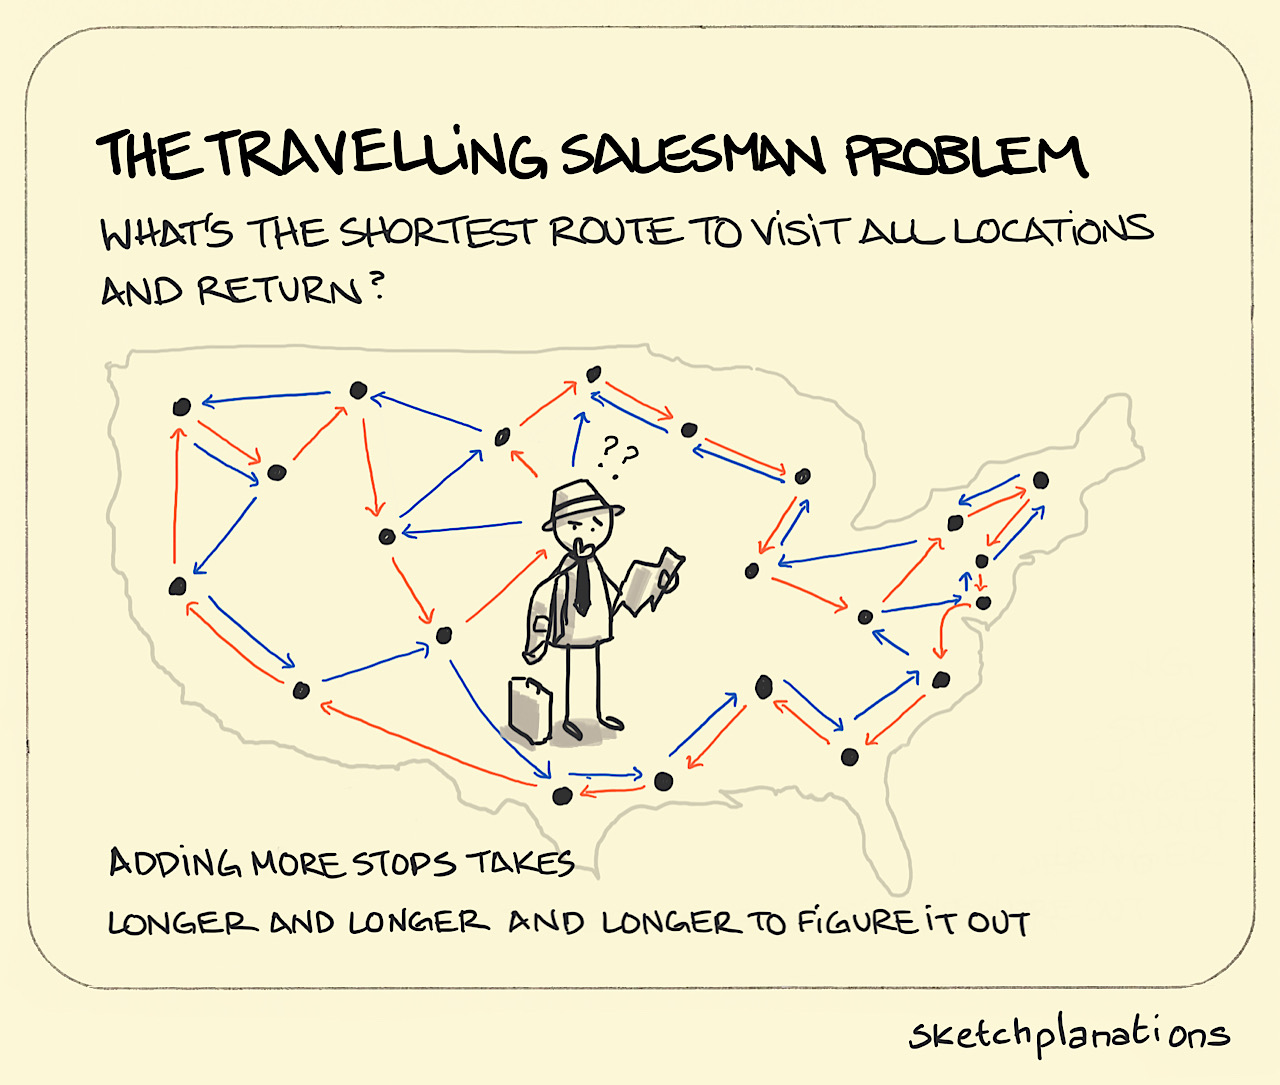
\includegraphics[width=1\textwidth]{CoverPhoto.jpg}
    \vspace{1cm}
    
    % NO PAGE NUMBER
    \thispagestyle{empty}
\end{titlepage}

\section*{Defining the problem}
\begin{center}
    \vspace{0.5cm}
    {\Large\itshape Introduction To Our Case Study\par}
\end{center}
Throughout this paper I will be making references to a theoretical Salesman.
The details of what they are selling is irrelevant for our topic so imagine that detail at your own discretion.
Our Salesman has one goal, visit every location at least once on a map and return home in the shortest possible time.
Finding the correct path varies upon the layout of locations (towns) to visit and how many of these exist. \\
\vspace{0.5cm}
A graph (map) with trivial result can be seen here:\\
\vspace{0.5cm}
INSERT TRIVIAL CASE OF TSP\\
\vspace{0.5cm}
Comparatively to this non-trivial result:\\
\vspace{0.5cm}
INSERT MEAN CASE OF TSP


\begin{center}
    %\vspace*{3cm}
    %{\Huge\bfseries Defining the problem\par}
    \vspace{0cm}
    {\Large\itshape Big O-Notation\par}
\end{center}
Our Salesman can go to many different towns in whichever order they wish.
The order however will impact the speed at which they can complete the task.
This is the rationale behind finding the shortest path.
Think back to our trivial case for the salesman from their introduction.
Now instead of traversing across the line we loop back repeatedly, using more steps than neccesary.
Whilst this will still allow the salesman to complete their rounds they will have missed dinner and be very upset.
Similarly, the time taken depends not just on the method, but also on who the Salesman is and if they have a faster van than a different one.
These human and environmental factors make it impossible to measure an algorithm's speed purely in seconds.
To address this, computer scientists use \textbf{Big O notation}, a mathematical way to describe how the number of steps an algorithm takes grows with the size of the input.
For example, an algorithm with complexity $O(n)$ will perform at most a number of operations proportional to the length of the input list ($n$).
An algorithm with $O(n^2)$ complexity might check each item against every other, leading to significantly more steps.
These expressions describe the algorithm’s \textbf{asymptotic behaviour} - that is, how it scales as inputs grow very large.
When this growth follows a polynomial pattern like $O(n)$ or $O(n^2)$, we say it runs in \textbf{polynomial time}, which is generally considered efficient and tractable.

\begin{center}
    \vspace{0cm}
    {\Large\itshape Sets and Set Notation\par}
\end{center}
Earlier, we used a salesman traversing across a map to explore algorithmic strategies.
Mathematically, the list of towns can be viewed as a \textbf{set} - a well-defined collection of distinct objects.
In computer science and mathematics, Sets are fundamental.
A set can contain numbers, items, states, algorithms, or even other sets.
For example, the set of paths include every possible route our salesman could take.
The set of solutions to a problem includes all algorithms that solve it.
We describe relationships between sets and their elements using \textbf{Set notation}:
\begin{itemize}
    \item $\in$: “is an element of” (e.g., $3 \in \{1, 2, 3\}$ means 3 is in the set)
    \item $\notin$: “is not an element of” (e.g., $4 \notin \{1, 2, 3\}$)
    \item $\subseteq$: “is a subset of” (e.g., $\{1,2\} \subseteq \{1,2,3\}$)
    \item $\cup$: union (e.g., $A \cup B$ contains all elements in $A$ or $B$)
    \item $\cap$: intersection (e.g., $A \cap B$ contains only elements in both $A$ and $B$)
    \item $\setminus$: set difference (e.g., $A \setminus B$ contains elements in $A$ but not in $B$)
\end{itemize}

\begin{center}
    \vspace{0cm}
    {\Large\itshape P\par}
\end{center}
The first set in our investigation is called \textbf{P}.
This set contains all problems that can be solved by an algorithm in \textbf{polynomial time} - meaning the number of steps required grows at most like $n$, $n^2$, $n^3$, etc., where $n$ is the size of the input.
A good example is the weekly shop.
Planning the optimal route through the store may take time, but it is feasible to compute in polynomial time - for example, with an algorithm of complexity $O(n^2)$.

\begin{center}
    \vspace{0cm}
    {\Large\itshape NP\par}
\end{center}
The (potentially larger) set \textbf{NP} stands for \textbf{nondeterministic polynomial time}. This set contains all problems where a proposed solution can be \textit{verified} in polynomial time, even if finding that solution might be difficult.
Consider back to our salesman: For non-trivial cases of the problem finding the optimal path is \( O(n^2 2^n) \).
Meaning right now we cannot solve it in polynomial time, but it can be verified in such time.
We know that $P \subseteq NP$: any problem we can solve efficiently, we can also verify efficiently.
Whether or not these sets are actually equal is the essence of our central question.

\begin{center}
    \vspace{0cm}
    {\Large\itshape Our Question\par}
\end{center}
This brings us to our guiding problem: \textbf{What is the relationship between $P$ and $NP$?}
Mathematically, we know that $P$ is a subset of $NP$, but we do not know whether $P = NP$. That is, we don't know whether every efficiently verifiable problem can also be efficiently solved.
Some mathematicians believe $\mathbf{P = NP}$ - implying that every hard-looking problem has a hidden efficient solution - while others believe $\mathbf{P \neq NP}$, suggesting some problems are inherently hard to solve even if easy to check.
This project does not aim to resolve the question. Instead, we will explore \textit{why} it has remained unanswered for decades - and examine the theoretical barriers that prevent us from settling it.
\vspace{4cm}

\section*{Relativization}
\begin{center}
    \vspace{0cm}
    {\Large\itshape Introduction to Relativization\par}
\end{center}
One of the most important—and possibly oldest—barriers to resolving \textit{P vs NP} is known as \textit{relativization}.
This idea was first formalized by three mathematicians in 1975, showing that a large group of mathematical proof methods face a fundamental limitation.
This limitation lies in their inability to separate the complexity classes discussed earlier when introducing \textit{Big O Notation}.
At its core, relativization involves measuring how these complexity classes behave when given access to an \textit{Oracle} (explored next), and how an algorithm's reasoning encounters a limit when this additional power is introduced.

\begin{center}
    \vspace{0cm}
    {\Large\itshape Oracles\par}
\end{center}
As defined by \cite{arora2009}:\\
Much like the legendary Oracle of Delphi, an \textit{Oracle} in complexity theory can provide an instant solution to a given subproblem.
It is an abstract tool—considered a 'black box'—that never reveals how it reaches its answer, only that it does.
We refer to any \textit{Turing Machine} with access to such a tool as an \textit{Oracle Turing Machine}, which may query the oracle at any point during computation.
A relatable instance could be whilst driving you use a GPS, this tool does not show you how it gets it's result however you will tend to trust it.
In that moment, using this information to guide your solution makes you behave almost like an \textit{Oracle Turing Machine}.
We denote this formally as $\mathbf{P^A}$ or $\mathbf{NP^A}$, meaning class $\mathbf{P}$ (or $\mathbf{NP}$) relative to oracle $A$.

\begin{center}
    \vspace{0cm}
    {\Large\itshape How does it apply to a resolution?\par}
\end{center}
A proof technique is said to \textit{relativize} if the logic of the proof still holds when both complexity classes are given access to the same oracle.
However, relativization as a method cannot resolve questions like $\mathbf{P = NP}$, as shown by Baker, Gill, and Solovay \cite{baker1975relativizations}.\\
They constructed two oracles, $A$ and $B$, such that:
\begin{itemize}
    \item $\mathbf{P^A = NP^A}$ (i.e., relative to oracle $A$, $\mathbf{P}$ and $\mathbf{NP}$ are equal)
    \item $\mathbf{P^B \neq NP^B}$ (i.e., relative to oracle $B$, they are distinct)
\end{itemize}
This demonstrates that any proof method which relativizes will yield inconsistent results depending on the oracle.
Consequently, such techniques cannot be used to resolve \textit{P vs NP}, because they fail in certain relativized scenarios.
This eliminates a large class of approaches and shows that any successful proof must go beyond relativization.

\begin{center}
    \vspace{0cm}
    {\Large\itshape Reflection\par}
\end{center}
As \cite{aaronson2005philosophers} argues, relativization reflects a deeper philosophical boundary.
Just as some truths lie beyond formal proof, some complexity class separations may lie beyond the reach of techniques that relativize.

\section*{Natural Proofs}
\begin{center}
    \vspace{0cm}
    {\Large\itshape Introduction to Natural Proofs\par}
\end{center}

Simply put, a \textit{Natural Proof} is a method that works on many different functions and is easy to apply.  
A property $\mathcal{P}$ is said to be \textbf{natural} if:
\begin{itemize}
    \item \textbf{Constructivity}: Given the truth table of a Boolean function $f$, we can determine whether $f \in \mathcal{P}$ in polynomial time.
    \item \textbf{Largeness}: A non-negligible portion of all Boolean functions satisfy $\mathcal{P}$.
\end{itemize}
This is best described by analogy.  
Imagine you're an English teacher - a strict one - who sets an essay for homework every lesson. You begin to suspect several students are using AI to write their essays.  
To catch them, you develop an algorithm that detects AI-generated writing. Maybe it looks for excessive use of em-dashes or unnatural phrasing.
This algorithm is simple and can be applied to \textit{every} essay you mark.  
However, once students realise how it works, they adapt their writing style to evade detection.  
This captures the flaw with Constructivity: if your method is too effective and too public, it can be countered.
Largeness suffers a related issue. If your detection method works on too \textit{many} types of cheating - copied essays, paraphrasing, ChatGPT, etc. - then you're likely catching even legitimate work, or again being too general to be reliable.
\vspace{1cm}
\newline
We care whether a proof is \textit{natural} because many known lower-bound techniques are.  
This becomes especially relevant when we're trying to prove the \textit{lower bound} of a function $f$ — that is, the fastest possible way to compute $f$.  
If we can do this, we may be able to show that $f \notin \mathbf{P}$.

\begin{center}
    \vspace{0cm}
    {\Large\itshape Circuit Complexity\par}
\end{center}
Before diving deeper into the limitations of Natural Proofs, we must take a step back and understand one of the main battlegrounds for proving $\mathbf{P \ne NP}$ - \textbf{circuit complexity}.
Refer to our Salesman.
Suppose instead of solving each map manually, they could build a dedicated machine for each map size - a custom calculator of sorts made entirely of logic gates (AND, OR, NOT).
This machine would take a list of towns and output the shortest route.
In computational terms, this machine is a \textbf{Boolean circuit}.
Circuits don't run sequentially like an algorithm.
They are a set arrengement of gates that perform a binary operation.
Each value of $n$ gets a seperate circtuit.
We intend to keep these circtuits small.
If we can prove that no small circuit can satisfy a problem we have proven that the problem does not lie in $P$.
In doing so proving $\mathbf{P \ne NP}$.
\vspace{0.2cm}
\textbf{Formally:}
The \textit{circuit complexity} $C(f)$ of a Boolean function $f : \{0,1\}^n \rightarrow \{0,1\}$ is the size of the smallest Boolean circuit that computes $f$ correctly on all inputs.
\vspace{0.1cm}
Referring back to our Salesman, if th4 smallest circuit they can build for the TSP grows faster than any polynomial in $n$, this proves that we need \textit{super-polynomial} resources.
This would strongly suggest $\mathbf{P \ne NP}$.
\vspace{0.2cm}
Despite decades of mathemeticians attempting to prove the lower bounds of problems in $\mathbf{NP}$, it has proven difficult.
Many of the proof techniques used are considered \textit{Natural}.
\begin{quote}
    "If we can prove that no small circuit solves a problem, we show that even the smartest shortcut-the most efficient mental 'machine'—won't help our Salesman beat the clock."\\
    - Inspired by  \cite{fortnow2009status}
\end{quote}

\begin{center}
    \vspace{0cm}
    {\Large\itshape Pseudorandom Functions\par}
\end{center}
Pseudorandom Functions (PRFs) are a core idea in cryptography.  
They are functions that look random, but are actually completely deterministic.  
To anyone without the secret key, the outputs seem unpredictable - even though they're generated by a fixed rule.
This idea is essential for secure communication.  
If you can't tell the difference between a random number and one generated by a PRF, then you also can't reverse-engineer passwords, decode messages, or guess encryption keys.
Here's the link to Natural Proofs:  
If you had a proof method that could tell whether a function was “hard” (i.e., had no small circuit), and that method was both constructive and large - then it could also be used to tell **whether a function was pseudorandom**.
This would be catastrophic. 
The ability to tell whether something is pseudorandom is exactly what modern cryptography tries to prevent.
So, if PRFs exist - and almost every encryption system assumes they do - then Natural Proofs can't work.  
They're too strong.  
They don't just solve $P \neq NP$ - they break the internet along the way.

\begin{center}
    \vspace{0cm}
    {\Large\itshape Razborov Rudich Insight\par}
\end{center}
In 1994, Alexander Razborov and Steven Rudich published a result that fundamentally changed how we think about proving lower bounds \cite{razborov1994}.
They showed that if secure pseudorandom functions exist - something almost all of cryptography relies on - then Natural Proofs cannot be used to separate $\mathbf{P}$ from $\mathbf{NP}$.
This was a shock.
Many earlier techniques for proving circuit lower bounds turned out to be \textit{natural} - they were efficient to check and applied to a wide range of functions.  
But Razborov and Rudich proved that any such natural method could be turned against cryptography: it would allow you to distinguish a pseudorandom function from a truly random one.
That's not just proving $\mathbf{P \ne NP}$.
That's breaking encryption.  
Since we assume pseudorandom functions exist, it must mean that \textbf{natural proofs can't work} - not because they're weak, but because they're too powerful.
As summarised in \cite{arora2009}, if a proof method is constructive and large, and still manages to prove a circuit lower bound for functions in $\mathbf{NP}$, it must also contradict the existence of pseudorandom functions.
This means that the search for new lower-bound techniques must avoid being \textit{natural} in this precise technical sense - a significant restriction.

\begin{center}
    \vspace{0cm}
    {\large\itshape An Analogy\par}
\end{center}
Imagine you're running airport security.  
You build a fast, effective scanner that flags any suspicious-looking bag based on known patterns - \textit{density, shape, wiring}.
It's fast enough to run on every passenger and catches most known threats.
This is your \textit{constructive} and \textit{large} method.
But what if attackers knew exactly how your scanner worked?  
They could design luggage that looks perfectly normal to your algorithm - even if it's dangerous.
Now, imagine someone builds a new scanner that works so well it catches even these disguised threats.
You get excited: maybe this new system will finally make flying totally safe.
But then someone points out a terrifying implication:  
\textit{If this scanner works as described, it would also catch military stealth tech. Or diplomatic pouches. Or even encrypted test samples from trusted researchers.}
In short - the scanner is \textit{too good}.  
If it works, it breaks things it wasn't meant to break.
That's the heart of the \cite{razborov1994} result.
If your method is constructive (efficient) and large (applies broadly), then it's strong enough to detect pseudorandom functions - which modern cryptography says you shouldn't be able to do -\cite{arora2009}.  
So unless we want to throw out the internet, these proof methods can't work.

\begin{center}
    \vspace{0cm}
    {\Large\itshape Consequences of a Natural Barrier\par}
\end{center}
The Razborov-Rudich insight does not just crumble our hope of a proof.
It fundamanetally changes where we have to look for a proof for $\mathbf{P \ne NP}$.
Their proof showed us that any proof method that satisifies the criteria to be \textit{Natural} would allow us to distinguish between pseudorandom and random functions.
Something assured to be computationally impossible under standard cryptographic assumptions.
In short: if your proof techniques can work broadly and efficiently it is too broad to break the foundations of Cryptography.
So unless you are willing to fundamanetally shatter the foundations of the modern internet your technique cannot be sufficient.\\
This creates a barrier with serious consequences:
\begin{itemize}
    \item It disqualifies many previously successful proof techniques, especially those that proved circuit lower bounds for simpler problems.
    \item It suggests that if $\mathbf{P \ne NP}$ is true, then any successful proof must avoid being natural - it must violate either Constructivity, Largeness, or both.
    \item It highlights a surprising link between cryptography and complexity theory: breakthroughs in one domain may endanger assumptions in the other.
\end{itemize}
Return to our Salesman:
Imagine you try to expose their inefficiency by building a test, a kind of security scanner for bad routes.
But every time you make it strong enough to work, it starts scanning and breaking real-world encrypted data.
In trying to catch the Salesman, you've also accidentally hacked a bank.
The scanner is too powerful to be safely used.

\begin{quote}
    "Natural proofs aren't too weak to prove $\mathbf{P \ne NP}$ - they're too powerful.
    They solve more than they should, and in doing so, they violate assumptions we rely on elsewhere."\\
    - Adapted from \cite{razborov1994}
\end{quote}

This result doesn't resolve the central question - but it tells us something just as important:
If $\mathbf{P \ne NP}$, then the path to proving it must avoid a large class of techniques.
\vspace{3cm}
\section*{Prerequesites to Algebraization}
Please note to the reader that this section may repeat some existing topics however the topics below are vital to our final barrier that it will prove beneficial to remind ourselves of them in depth.

\begin{center}
    \vspace{0cm}
    {\Large\itshape Boolean Circuits... Again\par}
\end{center}
To recap:\\
Previously, we met our Salesman and imagined that they could build a machine to solve each map.
This machine is not a computer in our sense, it does not run lines sequentially.
Instead, it is a physical circuit composed of 'simple' logic gates like AND, OR, and NOT.
These gates are arranged in a fixed pattern to solve one specific problem.
This model is known as a \textbf{Boolean circuit}.
Each circuit is designed for a single input size $n$.
Therefore, a circtuit to solve 5 towns is different to 6.\\
This allows us to show that: No matter how ingenius we are, any circuit that solves a problem like TSP must be enormous, then we have shown the problem to be fundamentally difficult.
We call this proving a \textit{Lower Bound}
Allowing us to answer the question of "even with custom hardware, how complex is the problem?"
Boolean circuits have given us conctrete methods to measure difficulty.
But in order to develop this idea further researchers began looking for more flexible and powerful tools.
Leading us to Oracles.

\begin{center}
    \vspace{0cm}
    {\Large\itshape Relativization: algorithms with Oracles\par}
\end{center}
Our Salesman is struggling to find the best route.
Instead of working it out themselves, they have been given access to a magical helper that can answer a question at any given time.
This helper is called an \textit{Oracle}
An Oracle does not explainits logic.
Simply responds with a boolean value (True or False) instantly.\\
"Is this route shorter than that one?" --- False\\
This Oracle changes the rules of our problem entirely.
The Salesman has just became significantly more powerful.
They can now build strategies that would be too difficult to compute themselves with the aid of their new magical helper.
Within Computer science, we represent complexity classes like: $\mathbf{P^A}$ or $\mathbf{NP^A}$ - Meaning te class $\mathbf{P}$ or $\mathbf{NP}$ when given access to the Oracle $A$.
We then say that a proof relativizes if it works regardless of an Oracles presence.\\
There is a twist to this however.
In 1975, Baker, Gill, and Solovay showed that some oracles make $\mathbf{P = NP}$, and others make $\mathbf{P \ne NP}$ \citep{baker1975relativizations}.
That means any proof technique that still works no matter what Oracle you add — any technique that relativizes — can’t possibly settle the question. It gives contradictory results depending on the Oracle.
As noted by \cite{arora2009}, relativization "applies to many known techniques" and explains why "some previously promising approaches are unlikely to resolve $\mathbf{P \ne NP}$".
\begin{quote}
    “Relativizing techniques are too blunt — they treat all oracles equally, even when the truth depends on which Oracle you choose.”\\
    - Paraphrased from \cite{baker1975relativizations}
\end{quote}
So giving the Salesman a magic assistant makes them more powerful, it also reveals that many of our traditional methods of proof hit a ceiling, including those using Circuits.
If they \textit{relatavize} they cannot prove  $\mathbf{P \ne NP}$.
To proceed further, we need tools that \textit{don't relativize}.
This is where algebra begins to enter the spotlight,

\begin{center}
    \vspace{0cm}
    {\Large\itshape Arithmetization\par}
\end{center}
Our Salesman so far has used logic gates and Oracles, boolean values and rigid machinery.
What if they could see the problem in higher resolution?
Instead of responding with a shallow "yes" or "no", what if they responded with a graph to explore or a map to see.
This is the key concept behind \textbf{arithmetization}.
Whithin complexity theory, arithmetization means transforming a boolean function, into a polynomial over a non infinite range.
The goal is simple: turn rigid boolean logic into flexible algebra.
Because algebra is powerful.
With polynomials, we can interpolate values, check identities, and apply mathematical techniques that just don't work on pure logic.
It gives us tools that are smoother and more continuous, even when applied to discrete problems.
In the early 1990s this approach was considered revolutionary.
researchers proved that $\mathbf{IP = PSPACE}$ - a result that shattered the barrier of relativization by using artithmetization \citep{arora2009}.
Showing that some techniques, by stepping outside convention, could reach further than thought possible.
\textbf{Metaphorically:}
Imagine the GPS of our Salesman no longer is limited to just giving directions.
It can now overlay a detailed landscape as smooth curves.
Now you don't just know if a better path exists, they can estimate just how much better the new path is.
\begin{quote}
    “Arithmetization allows an algorithm to reason about a function not just at specific points, but everywhere in between — like turning a pixelated map into a continuous surface.”\\
    - Adapted from \cite[Ch. 20.4]{arora2009}
\end{quote}
This method does not parallel relativization, it is significantly ahead.
Yet, when we tried to combine this with Oracle access we discovered a new barrier.

\begin{center}
    \vspace{0cm}
    {\Large\itshape Oracles with Algebra\par}
\end{center}
We know Oracles provide instant boolean results.
We also know arithmetization allows algorithms to work with algebra instead of boolean logic. 
What happens if we combine these?
This is the general idea behind \textbf{algebrization}.
Suppose our Salesman now has a magic map - an oracle - that only answers binary questions.
But also shows them the shape of terrain.
It reveals curves and gradients, costs and optimisations all as algebraic information.
This new Oracle not only answers boolean problems it gives algebraic reasoning.
In technical language: the oracle has been extended to allow access to a low-degree polynomial that agrees with the function from boolean input.
The algorithm can now acces both the function and algebraic extension $\tilde{A}$.\\
\vspace{0.3cm}
This looked like the breakthrough we needed.
After all, arithmetization had led to the remarkable result $\mathbf{IP = PSPACE}$, even though that result doesn't relativize \citep{arora2009}.
Maybe combining these ideas could finally allow us to show $\mathbf{P \ne NP}$.
But this hope was short-lived.
In 2008, Arora, Barak, and Wigderson showed that even \textit{algebrizing} techniques hit the same wall \citep{arora2008algebrization}.
They constructed special oracles where:
\begin{itemize}
    \item $\mathbf{P^A = NP^A}$, and
    \item $\mathbf{P^B \ne NP^B}$
\end{itemize}
Meaning that any proof method that works when you give it an Oracle \textit{and} its algebraic extension - a method that \textit{algebrizes} - cannot resolve $\mathbf{P \ne NP}$.\\
\vspace{0.3cm}
\textbf{Metaphorically:}  
It's like giving the Salesman a magical map that doesn't just point the way - it paints the whole landscape in equations.
But even with this power, they still can't find a shortcut.
No matter how detailed the map becomes, it doesn't contain the secret.
\begin{quote}
    “Algebrization unifies the strengths of relativization and arithmetization — and shows their combined limits.”\\
    - Adapted from \cite{arora2008algebrization}
\end{quote}
For some, this result was sobering.
It showed us that even the most powerful techniques known may not be enough, even united.
If we are to solve $\mathbf{P \ne NP}$, we must discover a fundamentally new kind of idea.
And that is where we turn next: to the barrier itself.

\bibliographystyle{unsrtnat}
\bibliography{references}

\end{document}
